\section{Espaço Tridimensional}

É notório verificar que as abordagens de navegação autônoma de veículos
terrestres mais usuais se baseiam em grande parte na restrição de uma visão
planar do ambiente, ou seja, um mundo plano. De fato, isto simplifica os modelos
e é uma abordagem consciente das suas limitações em relação à fidelidade de
representação do mundo real. Para ambientes controlados e até mesmo problemas
reais restritos a abordagem planar é bem sucedida. Já a abordagem tridimensional
é mais geral do que a abordagem planar pois descreve o espaço em todas as suas
reais dimensões. Portanto, ela contempla o caso planar como caso particular. Por
outro lado, inerentemente o custo computacional associado se torna mais elevado
devido aos aumento da complexidade e dimensionalidade dos modelos.

No que diz respeito a recursos computacionais, a computação embarcada atual já
viabiliza diversas aplicações onde modelos mais completos e complexos se tornam
praticáveis. Isto se traduz não só em maior realismo quando se trata da relação
com o utilizador do sistema como maior precisão devido aos modelos mais
completos. É neste sentido que as abordagens tridimensionais, no que diz
respeito à percepção do ambiente onde se inserem os robôs móveis, têm sido
buscadas pela comunidade científica atualmente.

A visão estéreo se insere neste contexto e é uma ferramenta para a extração da
informação tridimensional do ambiente. Os sensores laser tem desempenhado papel
importante na construção destes algoritmos por produzirem dados precisos a um
baixo custo computacional pois não há a necessidade de transformação do dado
capturado, como ocorre no caso das câmeras. Por outro lado são sensores
extremamente especializados, com características que por vezes limitam sua
aplicação real - são equipamentos sensíveis e geralmente não podem ser cobertos
por uma proteção, por exemplo. Câmeras de vídeo são de uso geral sendo
largamente utilizadas em diversas aplicações.

Conforme descrito na Seção \ref{sec:mapas_disparidade}, a partir de um conjunto
de câmeras através de uma visão estéreo é possível extrair informação visual do
espaço tridimensional do ambiente. Tais dados são convertidos em nuvens de
pontos (\fig{fig:nuvem_pontos}), e assim como para os sensores laser, os métodos
aplicados à interpretação e classificação se dão a partir destes pontos. Uma
nuvem de pontos nada mais é do que um conjunto de pontos no espaço sem
informação de correlação, apenas os dados de pontos no espaço. No caso das
câmeras, a informação cromática pode ainda ser agregada a estes pontos. Em
geral, as nuvens de pontos são classificadas de acordo com a sua densidade,
podendo ser esparsa ou densa. As câmeras apresentam outra vantagem por não só
produzirem pontos tridimensionais como provêem uma imagem do cenário, onde por
métodos de processamento de imagens e de visão computacional é possível extrair
diversas características que permitem uma interpretação da cena não
necessariamente tridimensional.

\vspace{0.5cm}

\begin{figure}[ht]
%	\centering
	\begin{minipage}[b]{0.33\linewidth}
	    \centering
	    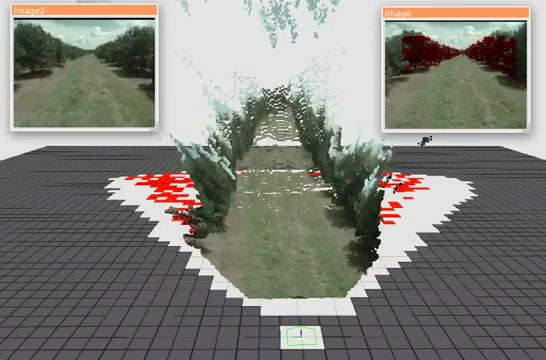
\includegraphics[width=\textwidth,height=4cm]{images/nuvem_pontos_caio.jpg}
	 	\caption{Nuvem de pontos a partir de câmera estéreo}
		\fonte{LRM (divulgação)}
	 	\label{fig:nuvem_pontos}
	\end{minipage}
	\begin{minipage}[b]{0.33\linewidth}
	    \centering
	    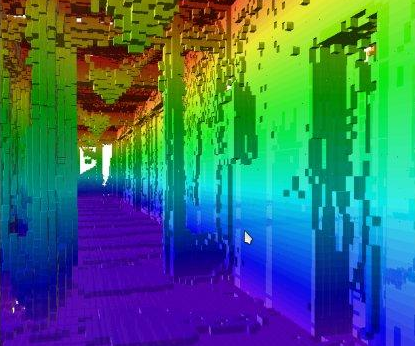
\includegraphics[width=\textwidth,height=4cm]{images/octomap.png}
	 	\caption{Mapa de ocupação (\textit{octomap})}
		\fonte{\\\cite{octomap}}
	 	\label{fig:octomap}
	\end{minipage}
	\begin{minipage}[b]{0.33\linewidth}
	    \centering
	    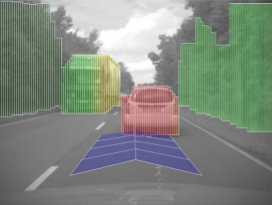
\includegraphics[width=\textwidth,height=4cm]{images/stixel.png}
	 	\caption{Segmentação por \textit{stixels}}
		\fonte{\cite{stixelworld}}
	 	\label{fig:stixel}
	\end{minipage}
\end{figure}

Devido à sua dimensionalidade, a informação a ser tratada é de ordem cúbica
comparada a ordem quadrática no caso planar. Algoritmos eficientes para tratar e
analisar tal volume de dados são necessários. O tratamento da informação deve
ser dado de forma volumétrica levando à necessidade de estruturas de dados
correspondentes. Largamente utilizado em computação gráfica, a representação por
\textit{voxels} é a abordagem tradicional pois permite discretizar o espaço em
sólidos cúbicos, reduzindo assim o espaço de busca. Uma técnica eficiente para a
representação de mapas tridimensionais é apresentada em \cite{octomap} e se
baseia no conceito de \textit{octrees}. Nesta abordagem o espaço é representado
por um \textit{octomap} (\fig{fig:octomap}), de acordo com a ocupação do espaço.
A informação da ocupação do espaço é obtida através de uma nuvem de pontos,
podendo esta ser fornecida de forma incremental, gerando então um mapa do espaço
de forma recursiva.

Outra abordagem de representação da informação tridimensional da cena em
agrupamentos por volumes é apresentada no trabalho de \cite{stixelworld}. Neste
trabalho é introduzido o conceito de \textit{stixel}, que representa um
determinado objeto a partir de sua projeção a partir do solo. O \textit{stixel}
é então um paralelepípedo (\fig{fig:stixel}) que representa uma região ocupada
na cena. Esta abordagem tem sido aplicada em reconhecimento de objetos na cena,
como veículos e pessoas \cite{Benenson2012}. O \textit{stixel} é dado por uma
base retangular e uma altura tendo o plano do chão como origem (representação
também chamada de 2,5 dimensões). Apesar de ser uma representação restritiva do
espaço tridimensional tem se demonstrado vantajosa principalmente em relação ao
seu custo computacional \cite{Benenson2011}.

%OSORIO
%> Ao final de cada capítulo sempre é bom ter uma seção de "Considerações
% Finais", na qual se faz uma reflexão do que foi apresentado (uma visão mais
% ampla de todo conteúdo) e aproveitando para fazer uma relação com o trabalho 
% como um todo e inclusive fazendo um "gancho" para o próximo capítulo

A construção e representação de mapas de ocupação por \textit{octree} se
apresenta mais vantajosa por ser uma representação estruturada dos dados,
enquanto os \textit{stixels} são independentes enquato estrutura de dados.
Porém, para classificação e clusterização de objetos na cena os \textit{stixels} já são
uma representação apropriada. Desta forma, utilizar ambas abordagens vem sendo
estudado com o propósito de agregar ambas características em um mapa de
navegabilidade.


%2012-10-15 Lido parcialmente (pode ser mais desenvolvido)